\documentclass{llncs}
\usepackage{amssymb}
\usepackage{graphicx}
\usepackage[ruled,linesnumbered,boxed]{algorithm2e}
\usepackage{graphicx}
\usepackage{amsmath}
%\usepackage{mathtools}
%\usepackage{color}
\usepackage{tabularx}
\usepackage[colorlinks, linkcolor=blue, anchorcolor=blue, citecolor=green]{hyperref}
%\usepackage{booktabs}
\usepackage[table]{xcolor}
%\uespackage{colortbl}
\usepackage[tight,footnotesize]{subfigure}
\usepackage{fancyhdr}
\usepackage{lastpage}
\usepackage{layout}
\usepackage{appendix}
%\usepackage{ctex}
\usepackage{float}
\usepackage{multirow}
\usepackage{booktabs}
\usepackage{comment}
\usepackage{enumerate}
\usepackage{algorithm2e}

\usepackage{indentfirst}
\setlength{\parindent}{2em}

%\footskip = 10pt
\pagestyle{fancy}
\chead{Group Project}
\lhead{CS7310-Algorithm@SJTU}
\rhead{Instructor: Xiaofeng Gao}
\rfoot{}
\cfoot{Page \thepage \ of \pageref{LastPage}}
\addtolength{\headheight}{0.5\baselineskip}
\addtolength{\headwidth}{0\marginparsep}
\addtolength{\headwidth}{0\marginparwidth}



\title{Resource Scheduling Problem in Hadoop}
\subtitle{\color{blue}{Project for Algorithm Design and Analysis} \vspace{-6mm}}

\author{
Xun Gong,\ 021033910012,\ gongxun@sjtu.edu.cn\\
Ning Yang,\ 021033910045,\ yn937391832@sjtu.edu.cn\\
Ziyu Wan,\ 021033910080,\ alex\_wan@sjtu.edu.cn
}
\institute{Department of Computer Science and Engineering, \\ Shanghai Jiao Tong University, Shanghai, China}

\begin{document}
\bibliographystyle{plain}
%\linespread{0.85}

%==============================================================================
\maketitle

\section*{Overview}

The problem of multi-core(job) resource scheduling has been studied for a long time. Researchers need to find an optimal schedule that minimize the \textit{makespan} or maximize the average utilization.
Though deterministic solutions for such a problem have been proved to be NP-hard, a variety of approximation methods with different properties and approximation ratios have been proposed.

The problem that we try to solve here is an variant in which we need make multi-level decisions on how to combine and allocate data blocks of each job onto different CPU cores of different hosts. In this problem, we cannot naively compute the speedup ratio as the number of cores used when executing a job but bear in our mind that the more cores we used, the more speed decay happens for a single core. Moreover, if we consider scheduling the jobs under multiple hosts settings, we should also take the time of data transmission into consideration.

During designing an efficient and effective algorithm, we've find some properties or limitations of this task. And by leveraging such properties or limitations, we've come up with some simple but very effective ideas which help us design good and practical algorithms finally.

For more convenient and accurate implementation, We refactored the code to the Python, and we use Python as our programming language for this project.

\subsection*{Properties and Limitations}
What we want to mention here at first is the design of speed decay for multi-core execution.
Given $n$ cores running one job together, the speed decay on each core is defined as
\begin{equation}
    g(n) = 1 - \alpha(n-1).
\end{equation}
We have two key observations about this setting:
\begin{enumerate}[(i.)]
    \item \textbf{More cores does not means better speedup ratio.}
    If we consider of the total speedup ratio of using $n$ cores which is $n(1 - \alpha(n-1))$, this is a quadratic function that have its maximum at $\displaystyle\frac{\alpha + 1}{2 \alpha}$. Take $\alpha=0.08$ for example, the above statement means that if we can distributed all data blocks of a job perfectly uniformly, we can get our theoretical optimal speedup ratio by using $n=7$ cores.
    
    \item \textbf{Very large number of cores even make negative speedups which is invalid and undefined.}
    From the definition of speed decay, we can find that if we the core number is too large, $n > \displaystyle\frac{\alpha + 1}{\alpha}$, we will get invalid speed since the decay factor becomes negative. This means we only need to consider at most a certain number of cores no matter how many cores there are when trying to run a job in parallel.
\end{enumerate}
Considering the above properties, we can easily find ways to accelerate and improve our algorithms.

\section*{Resource Scheduling for Single Host}
\subsection*{Problem formulation}
\textbf{Variables:} If index is not specified, we use $i$ is for job, $j$ is for core, $k$ is for data block.
Except those defined in the documentation, we define some new symbols as below:\\
$\omega \ge 0$ is the time when all jobs are done which is a positive real number.\\
$x_{i,j,k}\in[0,1]$is binary indicator of whether block $k$ of job $i$ allocated to core $j$\\
$y^i_j\in[0,1]$ is binary indicator of whether some block of job $i$ allocated to core $j$.\\
$sp_i > 0$ is the speed of job $i$.

\textbf{Constraints:} To satisfy the requirements, we should add the following constraints:
\begin{enumerate}[a.)]
    \item The time when all jobs are done must be greater than or equal to all jobs' finish time.
    \begin{equation}
        \omega \ge tf(job_i), \forall job_i
    \end{equation}
    
    \item The finish time of a job must be greater than or equal to the finish time of all cores for that job.
    \begin{equation}
        t_i + tp_j^i = tf_j^i \le tf(job_i), \forall job_i, c_j
    \end{equation}
    
    \item If two jobs share CPU cores, they must be executed in a strict order, namely one must be executed before/after the other one on that cpu core.
    \begin{equation}
        % \forall i_1 \ne i_2 \in J, \sum_{c_j}y_j^{i_1} \cdot y_j^{i_2} > 0, t_{i_1} < t_{i_2} \rightarrow z_{i_1} \le t_{i_2}
        y_j^{i_1}y_j^{i_2} (t_{i_1} - t_{i_2})(tf_j^{i_1} - t_{i_2}) \ge 0, \quad \forall job_{i_1} \ne job_{i_2}, c_j, 
    \end{equation}
    
    \item y should be harmonic with $x$.
    \begin{equation}
        y_j^i \ge x_{i,j,k} \quad \forall job_i, c_j, b^i_k
    \end{equation}
    
    \item all data blocks must be allocated to exactly one CPU core.
    \begin{equation}
        \sum_{c_j} x_{i,j,k} = 1. \quad \forall job_i, b^i_k
    \end{equation}
    
    \item The processing time of a job $i$ on core $j$ is must be the sum of data blocks allocated to it divides its speed.
    \begin{equation}
        \sum_{b_k^i} (x_{i,j,k} \cdot size(b_k^i)) = tp_j^i \cdot sp_i \quad \forall c_j, job_i
    \end{equation}
    
    \item The speed of each job must satisfy the project's requirements.
    \begin{equation}
        s_i \cdot (1 - \alpha \cdot (\sum_{c_j}y_j^i - 1)) \le sp_i
    \end{equation}
\end{enumerate}


\textbf{Objective} we use the objective in the documentation to find a schedule that minimize the finish time of the last job, i.e.
\begin{equation}
    \min \omega
\end{equation}


\subsection*{Solution}
Here we discuss our solution.
\subsubsection*{Method}
We propose to use greedy algorithms to schedule resource allocation. And we've tried some alternatives.

\begin{enumerate}
    \item Use only a single core for each job, then the problem becomes a Job Scheduling problem and we can use a sequential algorithm with approx. ratio about $\frac{4}{3}$.
    
    \item Sort all jobs to make their time of using single core in non-increasing order. Then each time pick a job and try to allocate as much cores as possible.
    
    \item Sort all jobs to make their time of using single core in non-increasing order. Set the maximal number of cores a job can use, $M$.
    Each time pick a job $i$ in the sorted list and then compare the bubble time of allocating it to $M$ cores and the bubble time of allocating $i$ and $(i+1)$ to $M$ cores(which is $M$ possible cases), if the former is smaller, choose the one with smaller bubble time and allocate next jobs.
    
    \item Enumerate the maximum number of jobs in parallel, $m_j$. Sort all jobs to make their time of using single core in non-increasing order in a queue.
    Each time pop the first $m_j$ jobs and allocate these jobs on almost equivalent number of cores.
    Then pick the optimal $m_j$.
\end{enumerate}

\subsubsection*{Pseudocode}
In our experiments generated under multiple hyper-parameters, we found that the last algorithm has best performance in average. So we only show its pseudocode \ref{alg-singlehost} and analyze it.

\begin{algorithm}[htbp]
  \KwIn{$\{c_j\}_j$, $\{jobs_i\}_i$, $\{b_k^i\}_k^i$, $\{s_i\}_i$}
  \KwOut{A schedule of resource allocation}
  \BlankLine
  \caption{Greedy Schedule on Single Host} \label{alg-singlehost}
  
  SC\_OPT=None, T\_OPT=$\infty$\;
  \For{$job \in J$  with index $i$}{
        Sort the blocks of job $i$ decreasingly according to their data size\;
        \For{$j=1$ to $|C|$}{
            compute $EndTime[i][j]$ as the shortest time using $j$ cores for job $i$ with sequential algorithm\;
        }
  }
    
  Sort $J$ according to their total data block size divides their speed in non-increasing order\;
  \For{$np=1$ to $|C|$} {
    \For{$job \in J$  with index $i$}{
        compute $nc$ as used for this job as \#core $= \min[\arg\min_j EndTime[i][j]\ ,\ floor({\frac{|C| + i \mod np}{np}})]$\;
        pick $nc$ cores with minimal finish time as $U$\;
        
        \For{$b_k^i \in B^i$ in a non-increasing order} {
            find the core $c\in U$ with minimal finish time\;
            put $b_k^i$ on $c$\;
        }
    }
    \uIf{Current schedule's finish time is better then T\_OPT}{
        SC\_OPT= current schedule\;
        T\_OPT = current schedule's finish time\;
    }
  }
  \KwOut{SC\_OPT, T\_OPT} \;
\end{algorithm}

\subsubsection*{Complexity Analysis}
The time complexity is analyzed in Table.\ref{tab-singlehost-complexity}

\begin{table}[t]
\caption{Time Complexity for single-host algorithm}
\begin{center}
\begin{tabular}{c|c}
\toprule
\textbf{code lines} &\textbf{Time Complexity}  \\
\midrule
line $3$ & $O(|J| |B|\log |B|)$  \\
line $5$ & $O(|J| |C| |B|\log |B|)$  \\
line $8$ & $O(|J| |B| +  |J|\log |J|)$  \\
line $12$ & $O(|J| |C|^2 \log |C|)$\\
line $14$ & $O(|J| |C|^2 |B|)$  \\
\bottomrule
\end{tabular}
\label{tab-singlehost-complexity}
\end{center}
\end{table}

\subsubsection*{Case Study}
We present the visualization results of some test cases here and analyze our algorithm's behavior. Fig.\ref{fig:task1} shows the execution diagram of solution for given test case for single-host scheduling problem. In our optimal solution, almost all jobs are executed on a single core and such schedule brings a tiny amount of bubble. With up to $88.72\%$ utilization, we can come to the conclusion that our algorithm has good enough performance.

\begin{figure}[t]
    \centering
    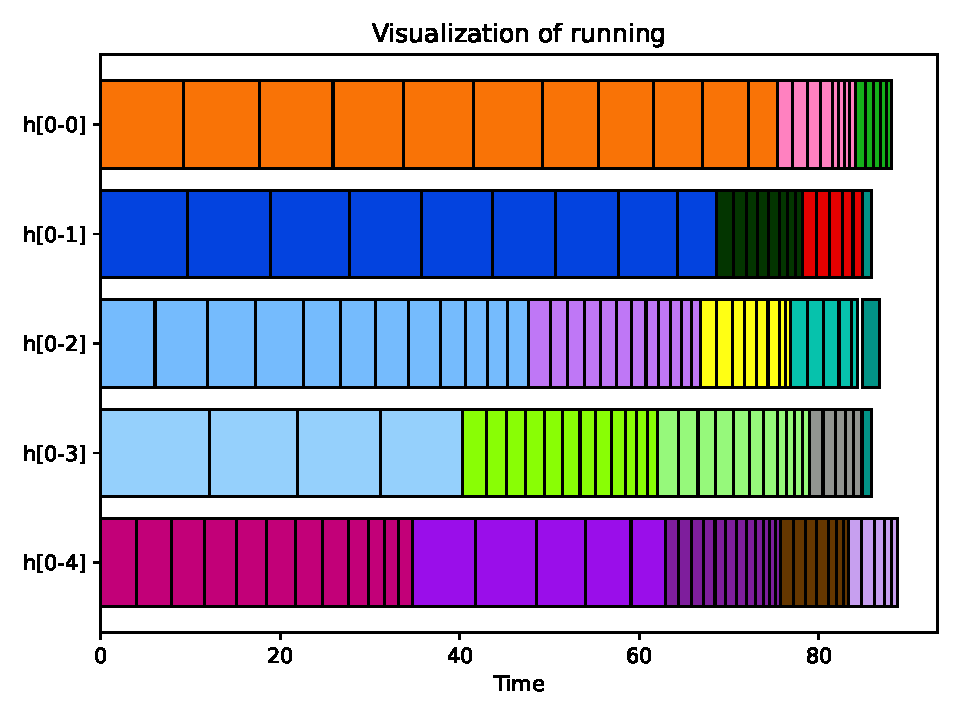
\includegraphics[width=0.9\textwidth]{task1.pdf}
    \caption{Visualization of test case for single host scheduling problem}
    \label{fig:task1}
\end{figure}

Moreover, we also present the visualization result for a larger test case generated randomly. As is shown in Fig.\ref{fig:task1_random}, all data blocks have been tightly arranged as a rectangle resulting in few amount of bubbles which means our algorithm find an efficient schedule for this test case. And the $98.7\%$ utilization means not only our algorithm is powerful but also the metrics of utilization is not very reasonable as it should take all the bubbles into consideration.

\begin{figure}[htpb]
    \centering
    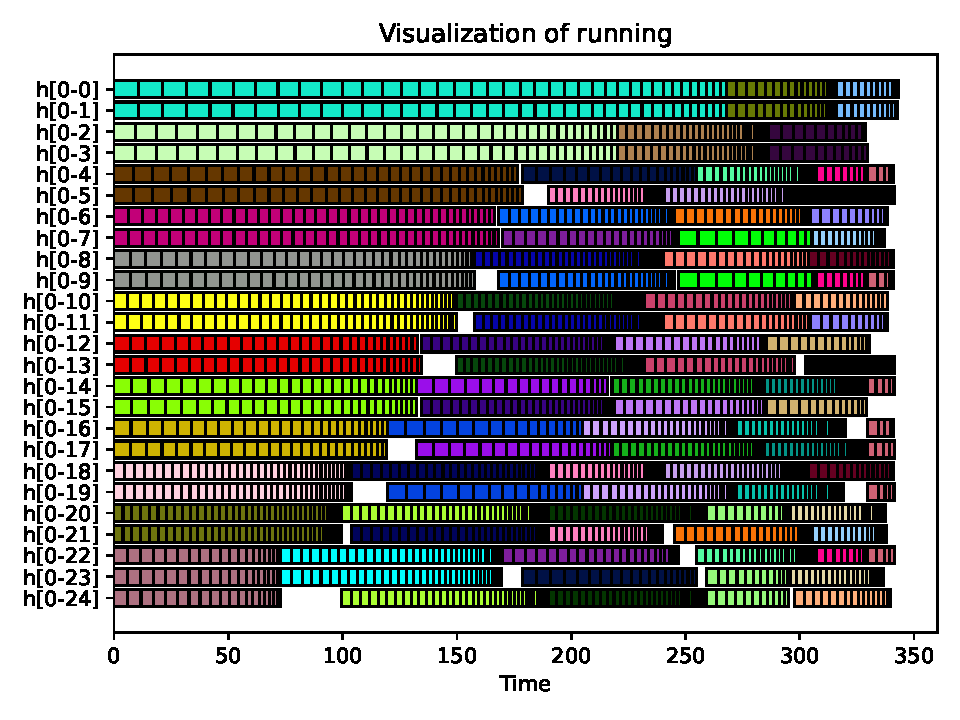
\includegraphics[width=0.9\textwidth]{task1_random_generate.pdf}
    \caption{Visualization of randomly generated test case for single host scheduling problem}
    \label{fig:task1_random}
\end{figure}

% --------------------------------------------------------------
% ------------------- END FOR SINGLE HOST ----------------------
% --------------------------------------------------------------
\newpage
\section*{Resource Scheduling for Multiple Hosts}
\subsection*{Problem formulation}
\textbf{Variables:} If index is not specified, we use $i$ is for job, $j$ is for core, $k$ is for data block.
Except those defined in the documentation, we define some new symbols as below:\\
$\omega \ge 0$ is the time when all jobs are done which is a positive real number.\\
$z_i \ge 0$ is the finish time of job $i$, which is a positive real number.\\
$x_{i,j,k,l}\in[0,1]$is a binary indicator of whether block $k$ of job $i$ allocated to core $j$ on host $l$\\
$y^i_{j,l}\in[0,1]$ is a binary indicator of whether some block of job $i$ allocated to core $j$ on host $l$.\\
$sp_i > 0$ is the speed of job $i$.\\
$ts_{i,j,l}\ge 0$ is the time of transmission of job $i$ to core $j$ on host $l$.\\
$loc_{k,l}^i \in [0, 1]$ is a binary indicator of whether the initial location of block $k$ of job $i$ is host $l$.\\

\textbf{Constraints:} To satisfy the requirements, we should add the following constraints:

\begin{enumerate}[a.)]
    \item The time when all jobs are done must be greater than or equal to all jobs’ finish time.
    \begin{equation}
        \omega \ge tf(job_i), \quad \forall job_i
    \end{equation}
    
    \item The finish time of a job must be greater than or equal to the finish time of all cores on all hosts for that job.
    \begin{equation}
        t_i + tp_{l,j}^i = tf_{l,j}^k \le tf(job_i)
    \end{equation}
    
    \item If two jobs share CPU cores, they must be executed in a strict order, namely one must be executed before/after the other one on that CPU core.
    \begin{equation}
        y_{j,l}^{i_1}y_{j,l}^{i_2}(t_{i_1} - t_{i_2})(tf^{i_1}_{j,l} - t_{i_2}) \ge 0, \quad \forall job_{i_1} \ne job_{i_2}, c_j, h_l
    \end{equation}
    
    \item $y$ should be harmonic with $x$.
    \begin{equation}
        y_{j,l}^i \ge x_{i,j,k,l}, \quad \forall job_i, c_j^l, b^i_k, h_l
    \end{equation}
    
    \item all data blocks must be allocated to exactly one CPU core
    \begin{equation}
        \sum_{c_j, h_l} x_{i,j,k,l} = 1, \quad \forall job_i, b_k^i
    \end{equation}
    
    \item The processing time of a job $i$ on core $j$  must be the sum of data blocks allocated to it divides its speed plus the time of transmission.
    \begin{equation}
        \sum_{b^i_k} (x_{i,j,k,l} \cdot size(b_k^i)) / sp_i + ts_{i,j,l} = tp_{j,l}^i,\quad job_i, c_j^l, h_l
    \end{equation}
    
    \item The speed of each job must satisfy the project’s requirements.
    \begin{equation}
        0 < s_i \cdot (1 - \alpha \cdot (\sum_{c_j, h_l}y_{j,l}^i - 1)) \le sp_i
    \end{equation}
    
    \item The time of transmission must satisfy the project's requirements.
    \begin{equation}
        \sum_{b_k^i} \left[ x_{i,j,k,l} \cdot (x_{i,j,k,l} - loc^i_{k,l}) \cdot size(b_k^i) \right]= ts_{i,j,l} \cdot s_t, \quad \forall job_i, h_l, c_j^l
    \end{equation}
\end{enumerate}

\textbf{Objective} we use the objective in the documentation to find a schedule that minimize the finish time of the last job, i.e.
\begin{equation}
    \min \omega
\end{equation}


\subsection*{Solution}
Here we discuss our solution.
\subsubsection*{Method}
We propose to use greedy algorithms to schedule resource allocation. And we've tried some alternatives.

It is worth noting that there is a feature where the transfer speed is much faster than the calculation speed of core for a given data range. So in most cases the benefits of transmission outweigh the costs of parallelism and transmission. To simplify the problem, the parallel benefits will be prioritized in the following algorithm.

\begin{enumerate}
    \item 
    Similar to Task 1, just consider use a single core fore each job, then the transmission time is almost fixed, which become an approximation of Job Scheduling of Single Host,
    
    \item
    In this algorithm, we use two tricks: first, we want to consider all the core at one host, and add corresponding transmission time on each block as running time, then arrange them to core with the earliest finish time. Second, because of the existence of the computing decaying coefficient $g(\cdot)$ \&, use core as many as possible may not get the optimal result. So we set a limitation for maximum number of parallel cores for a job, then explore this limitation for best result. A brief description as follow:
    
    Sort all the jobs by its sum of block size in non-increasing order, then consider all cores at one host, for each job, do a sorting to find which cores will be chosen to handle this job according to finish time and transmission time, then run a greedy algorithm to schedule jobs' blocks on these cores, at last update the parameters. This process will repeat for different maximum core limitation, and pick the optimal result.
    
    Intuitively speaking, this algorithm has considered the transmission time between host, whose result will be better than hadn't. But in the task2, we get better result without the consideration of transmission time. This phenomenon is counter-intuitive. A possible explanation is that transmission speed in this task is far more faster than calculation speed of core, so compare with saving transmission time, doing transmission to the core with earlier finish time will get better effect.
    
\end{enumerate}


\subsubsection*{Pseudocode}
In our experiments generated under multiple hyper-parameters, we found that the last algorithm has best performance in average. So we only show its pseudocode \ref{alg-multihost} and analyze it.

\begin{algorithm}[htbp]
  \KwIn{$\{c_j\}_j$, $\{jobs_i\}_i$, $\{b_k^i\}_k^i$, $\{s_i\}_i$}
  \KwOut{A schedule of resource allocation}
  \BlankLine
  \caption{Greedy Schedule on Multiple Host} \label{alg-multihost}
  SC\_OPT=None, T\_OPT=$\infty$\;
  
  Sort $J$ according to their total data block size divides their speed in non-increasing order\;
  
  $C* = \bigcup_{host \in H}\ \text{\{cores in h\}}$ \;
  
  \For{$job \in J$  with index $i$}{
        % Select cores
        Get $D^i_h$ as datasize for all blocks initialized in host $h$ \;
        
        Get maximize used \#cores $= \min(|B^i|, |C*|)$ \;
        
        Pick $\#$-earliest finished cores $U$ to use, across all possible cores by $\arg\min_{top-j} (tf_j - B^i_h / s_t)$ \;
        
        $s_i = s_i * (1 - \alpha * (|U| - 1))$ \;
        
        Sort the blocks $B^i$ of job $i$ decreasingly according to their data size and transmission penalty $\arg\max (size(B_j^i) / s_i)$ \;
        
        \For{Block $b_k^i$ in $B^i$}{
            Find the core $c \in U$ win minimal finish time \;
        
            Put $b_k^i$ on $c$ \;
        }
        \uIf{Current schedule's finish time is better then T\_OPT}{
            SC\_OPT= current schedule\;
            T\_OPT = current schedule's finish time\;
        }
  }
  
  \KwOut{SC\_OPT, T\_OPT} \;
\end{algorithm}

\subsubsection*{Complexity Analysis}
The time complexity is analyzed in Table.\ref{tab-multihost-complexity}

\begin{table}[t]
\caption{Time Complexity for multi-host algorithm}
\begin{center}
\begin{tabular}{c|c}
\toprule
\textbf{code lines} &\textbf{Time Complexity}  \\
\midrule
line $2$ & $O(|J| |B|\log |B|)$  \\
line $7$ & $O(|C| |B| \log |B| )$  \\
line $9$ & $O(|J| |B| \log |B|)$  \\
line $10$ & $O(|B| |C|^2)$\\
\bottomrule
\end{tabular}
\label{tab-multihost-complexity}
\end{center}
\end{table}


\subsubsection*{Case Study}

We present the visualization results of some test cases here and analyze our algorithm's behavior. Fig.\ref{fig:task2} shows the execution diagram of solution for given test case for multi-host scheduling problem. With given task2, our finish time is 44.89s, total response time is 670.21s, and our utilization rate can up to $98.1\%$, we can come to the conclusion that our algorithm has good enough performance.

Moreover, we generate some random case and based on our observation we have some conclusion: in our optimal solution, we enumerate the maximum core number to search better result, and we find that for a ideal arbitrarily divisible job, it uses 6 or 7 cores may get best result for itself; for the whole task, most job using 2-5 cores will get the global optimal result. Here we give a visualization result for a larger random-generated test case to prove this, as is shown in Fig.\ref{fig:task2_random}. The core used for each block is usually at most 4, and the algorithm try to spilt equally with blocksize to get the theoretically optimal situation, so we can see that there are hardly any bubble time in cores, and the utilization rate is $97.46 \%$, which shows that our algorithm has good expandability and generalizability. However, this algorithm did not fully consider the optimization of mixed quantity core, so it's still not optimal for sure, but it still a algorithm very close to real optimal solution.

\begin{figure}[t]
    \centering
    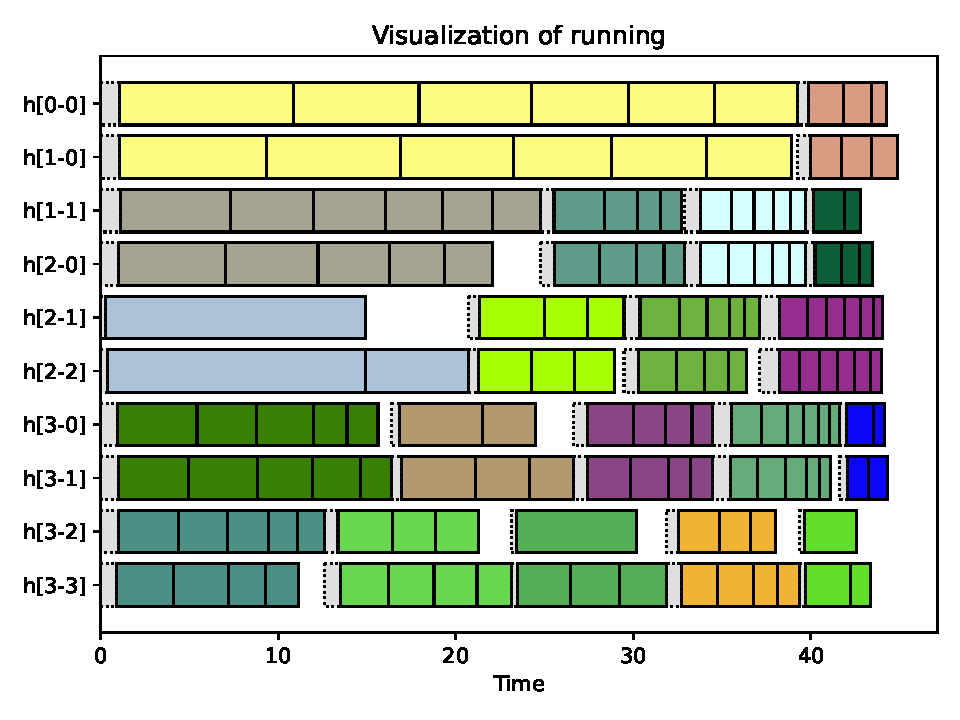
\includegraphics[width=0.9\linewidth]{task2.pdf}
    \caption{Visualization of the given test case for multi-host scheduling problem. Grey box is the data transmission.}
    \label{fig:task2}
\end{figure}

\begin{figure}[htbp]
    \centering
    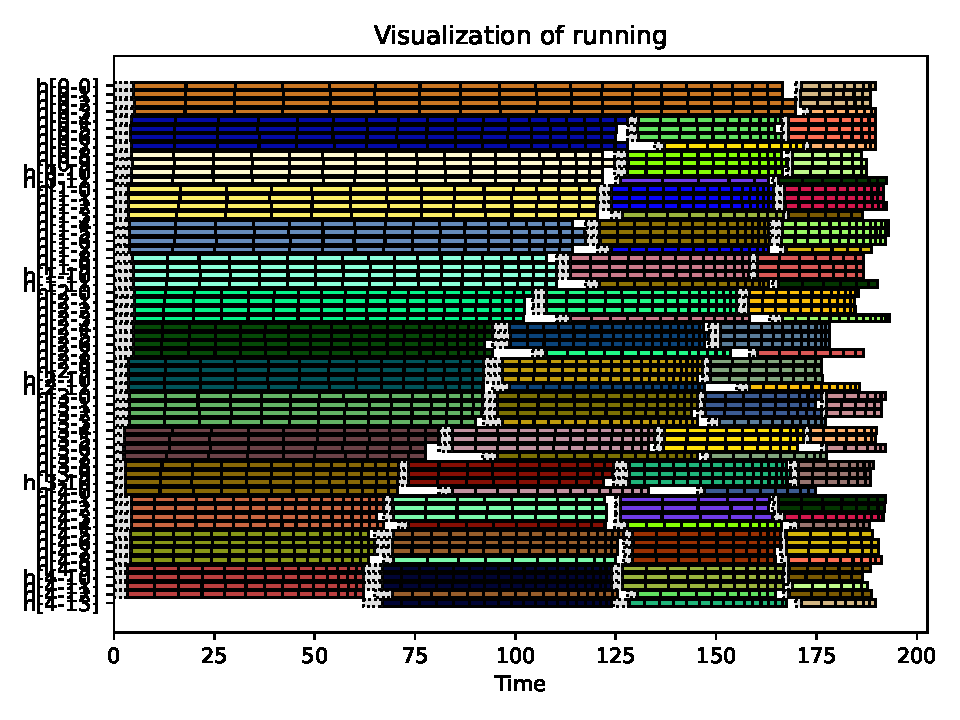
\includegraphics[width=\textwidth]{task2_random_generate.pdf}
    \caption{Visualization of randomly generated test case for multi-host scheduling problem. Grey box is the data transmission.}
    \label{fig:task2_random}
\end{figure}


\section*{Acknowledgements}
We thank for the teachers, TAs and students who give great support in completing this project.



% Here is your acknowledgements. You may also include your feelings, suggestion, and comments in the acknowledgement section.

%
% ---- Bibliography ----
%
% BibTeX users should specify bibliography style 'splncs04'.
% References will then be sorted and formatted in the correct style.
%
%\bibliographystyle{splncs04}
% \bibliography{refpaper.bib}
%



\newpage
\begin{appendices}
\section*{Appendix}

\begin{table}[htbp]
\caption{Symbols and Definitions}
\begin{center}
\begin{tabular}{c|c}
\toprule
\textbf{Symbols} &\textbf{Definitions}  \\
\midrule
$n$ & The number of jobs  \\
$m$ & The number of cores \\
$q$ & The number of hosts  \\
$job_i$, $J$ & $job_i$ is the $i$-th job. The job set is $J=\{job_0, \cdots, job_{n-1}\}$. \\
$h_l$, $H$ & $h_l$ is the $l$-th  host. The host set is $H=\{h_0, \cdots, h_{q-1}\}$. \\
$m_l$ & The number of cores on host $h_l$\\
$c^l_j$, $C_l$ & $c^l_j$ is the $j$-th core on host $h_l$. $C_l$ is the set of cores on host $h_l$.\\
$C$ & The set of cores. $C=\{c_0,\cdots,c_{m-1}\}$ for single-host. $C=\cup_{l=0}^{q-1} C_l$ for multi-host.\\
$b^i_k$& The block of $job_i$ whose id is $k$\\
$B^i_{j}$ & The set of data blocks of $job_i$ allocated to core $c_j$ \\
$B^i$ & The set of data blocks of $job_i$ \\
$B^i_{lj}$ & The set of data blocks of $job_i$ allocated to core $c^l_j$ \\
$B$ & The set of blocks of all jobs, $B = \bigcap_{i} B^{i}$ \\
$\widetilde{B}^i_{lj}$ & The set of data blocks of $job_i$ allocated to core $c^l_j$ but not initially stored on $h_l$\\
$size(\cdot)$ & The size function of data block\\
$g(\cdot)$ &  The computing decaying coefficient caused by multi-core effect\\
$s_i$ & The computing speed of $job_i$ by a single core\\
$s_t$ & The transmission speed of data \\
$e_i$ & The number of cores processing $job_i$\\
$t_i$ & The time to start processing $job_i$\\
$tp^i_j$, $tf^i_{j}$ & The processing time / finishing time of core $c_j$ for $job_i$\\
$tp^i_{lj}$, $tf^i_{lj}$ & The processing time / finishing time of core $c^l_j$ for $job_i$\\
$tf(job_i)$ & The finishing time of $job_i$ \\
$\omega$ & The time when all jobs are done, which is a positive real number.\\
$z_i$ & The finish time of job $i$, which is a positive real number.\\
$x_{i,j,k}$ & The binary indicator of whether block $k$ of job $i$ allocated to core $j$\\
$y^i_j$ & The binary indicator of whether some block of job $i$ allocated to core $j$.\\
%  & \\
%  & \\
%  & \\
%  & \\
%  & \\
%  & \\
\bottomrule
%\multicolumn{4}{l}{$^{\mathrm{a}}$Sample of a Table footnote.}
\end{tabular}
\label{tabSYMBOLS}
\end{center}
\end{table}




\end{appendices}

%\begin{comment}
%\begin{thebibliography}{8}
%\bibitem{ref_article}
%Author, F.: Article title. Journal \textbf{2}(5), 99--110 (2016)
% \bibitem{dean2008mapreduce}
% Dean J, Ghemawat S. MapReduce: simplified data processing on large clusters[J]. Communications of the ACM, 2008, 51(1): 107-113.

% \bibitem{ref_lncs1}
% Author, F., Author, S.: Title of a proceedings paper. In: Editor,
% F., Editor, S. (eds.) CONFERENCE 2016, LNCS, vol. 9999, pp. 1--13.
% Springer, Heidelberg (2016).

% \bibitem{ref_book1}
% Author, F., Author, S., Author, T.: Book title. 2nd edn. Publisher,
% Location (1999)

% \bibitem{ref_proc1}
% Author, A.-B.: Contribution title. In: 9th International Proceedings
% on Proceedings, pp. 1--2. Publisher, Location (2010)

% \bibitem{ref_url1}
% LNCS Homepage, \url{http://www.springer.com/lncs}. Last accessed 4
% Oct 2017
%\end{thebibliography}
%\end{comment}

\end{document}


